\section{Image\-Data Class Reference}
\label{class_c_s_image_viewer_1_1_image_data}\index{CSImageViewer::ImageData@{CSImageViewer::ImageData}}
class containing the actual pixel data values (note that this class is abstract)  


Inheritance diagram for Image\-Data::\begin{figure}[H]
\begin{center}
\leavevmode
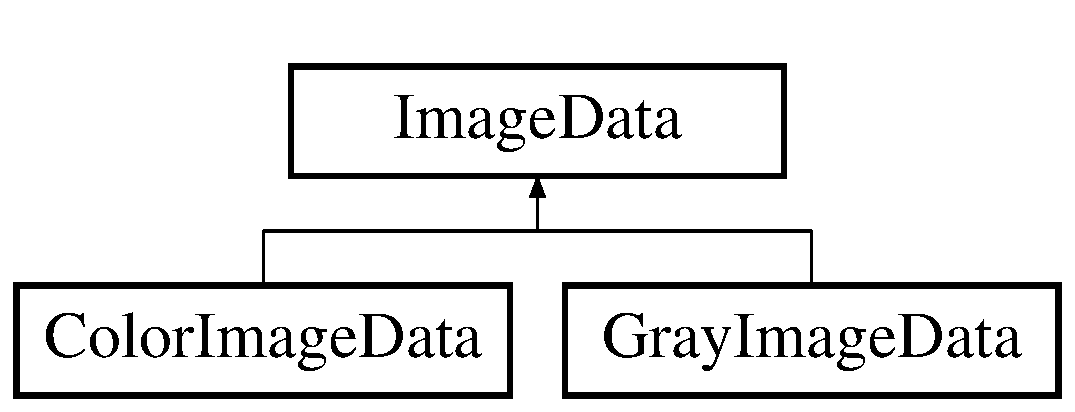
\includegraphics[height=2cm]{class_c_s_image_viewer_1_1_image_data}
\end{center}
\end{figure}
\subsection*{Public Member Functions}
\begin{CompactItemize}
\item 
void {\bf save\-Display\-Image} (String fname)
\begin{CompactList}\small\item\em Save the display image to a file. \item\end{CompactList}\item 
bool {\bf get\-Is\-Color} ()
\begin{CompactList}\small\item\em accessor returning whether this is a color (or gray) image. \item\end{CompactList}\item 
bool {\bf get\-Is\-Audio} ()
\begin{CompactList}\small\item\em accessor returning whether this is audio data. \item\end{CompactList}\item 
bool {\bf get\-Image\-Modified} ()
\begin{CompactList}\small\item\em accessor returning whether this image has been modified (changed) or not. \item\end{CompactList}\item 
int {\bf get\-W} ()
\begin{CompactList}\small\item\em accessor returning image width. \item\end{CompactList}\item 
int {\bf get\-H} ()
\begin{CompactList}\small\item\em accessor returning image height. \item\end{CompactList}\item 
int {\bf get\-Min} ()
\begin{CompactList}\small\item\em accessor returning min image value. \item\end{CompactList}\item 
int {\bf get\-Max} ()
\begin{CompactList}\small\item\em accessor returning max image value. \item\end{CompactList}\item 
int {\bf get\-Data} (int i)
\begin{CompactList}\small\item\em accessor returning specific pixel value in image (in original image data). \item\end{CompactList}\item 
String {\bf get\-Fname} ()
\begin{CompactList}\small\item\em accessor returning input image file name (if any). \item\end{CompactList}\end{CompactItemize}
\subsection*{Static Public Member Functions}
\begin{CompactItemize}
\item 
static {\bf Image\-Data} {\bf load} (String file\-Name)
\begin{CompactList}\small\item\em Given the name of an input image file, this method determines the type of image and then invokes the appropriate constructor. \item\end{CompactList}\end{CompactItemize}
\subsection*{Public Attributes}
\begin{CompactItemize}
\item 
int[$\,$] {\bf m\-Display\-Data}
\begin{CompactList}\small\item\em Possibly modified copy of m\-Original data that can be used for contrast changes, edge detection, filtering, etc. \item\end{CompactList}\item 
Bitmap {\bf m\-Display\-Image}
\begin{CompactList}\small\item\em image drawn on screen \item\end{CompactList}\end{CompactItemize}
\subsection*{Protected Attributes}
\begin{CompactItemize}
\item 
bool {\bf m\-Is\-Color}
\begin{CompactList}\small\item\em true if color (rgb); false if gray (or audio) \item\end{CompactList}\item 
bool {\bf m\-Is\-Audio}
\begin{CompactList}\small\item\em true if audio; false if color or ordinary gray \item\end{CompactList}\item 
bool {\bf m\-Image\-Modified}
\begin{CompactList}\small\item\em true if image has been modified \item\end{CompactList}\item 
int {\bf m\-W}
\begin{CompactList}\small\item\em image width \item\end{CompactList}\item 
int {\bf m\-H}
\begin{CompactList}\small\item\em image height \item\end{CompactList}\item 
int {\bf m\-Min}
\begin{CompactList}\small\item\em overall min image pixel value \item\end{CompactList}\item 
int {\bf m\-Max}
\begin{CompactList}\small\item\em overall max image pixel value \item\end{CompactList}\item 
String {\bf m\-Fname}
\begin{CompactList}\small\item\em (optional) file name \item\end{CompactList}\item 
int[$\,$] {\bf m\-Original\-Data}
\begin{CompactList}\small\item\em Actual original (unmodified) unpacked (1 component per array entry) image data. \item\end{CompactList}\end{CompactItemize}


\subsection{Detailed Description}
class containing the actual pixel data values (note that this class is abstract) 

This class contains the actual image pixel data. Note that this class is abstract. 



\subsection{Member Function Documentation}
\index{CSImageViewer::ImageData@{CSImage\-Viewer::Image\-Data}!getData@{getData}}
\index{getData@{getData}!CSImageViewer::ImageData@{CSImage\-Viewer::Image\-Data}}
\subsubsection{\setlength{\rightskip}{0pt plus 5cm}int get\-Data (int {\em i})}\label{class_c_s_image_viewer_1_1_image_data_484a091210aca6efdb70b5fa2083f978}


accessor returning specific pixel value in image (in original image data). 

\index{CSImageViewer::ImageData@{CSImage\-Viewer::Image\-Data}!getFname@{getFname}}
\index{getFname@{getFname}!CSImageViewer::ImageData@{CSImage\-Viewer::Image\-Data}}
\subsubsection{\setlength{\rightskip}{0pt plus 5cm}String get\-Fname ()}\label{class_c_s_image_viewer_1_1_image_data_c4573ecf419c7e5ee6940d80198ca053}


accessor returning input image file name (if any). 

\index{CSImageViewer::ImageData@{CSImage\-Viewer::Image\-Data}!getH@{getH}}
\index{getH@{getH}!CSImageViewer::ImageData@{CSImage\-Viewer::Image\-Data}}
\subsubsection{\setlength{\rightskip}{0pt plus 5cm}int get\-H ()}\label{class_c_s_image_viewer_1_1_image_data_9921a0a54c2b0b3948d1b914e88bd1d8}


accessor returning image height. 

\index{CSImageViewer::ImageData@{CSImage\-Viewer::Image\-Data}!getImageModified@{getImageModified}}
\index{getImageModified@{getImageModified}!CSImageViewer::ImageData@{CSImage\-Viewer::Image\-Data}}
\subsubsection{\setlength{\rightskip}{0pt plus 5cm}bool get\-Image\-Modified ()}\label{class_c_s_image_viewer_1_1_image_data_68c87c6f22371f3afa7e5e55edf80148}


accessor returning whether this image has been modified (changed) or not. 

\index{CSImageViewer::ImageData@{CSImage\-Viewer::Image\-Data}!getIsAudio@{getIsAudio}}
\index{getIsAudio@{getIsAudio}!CSImageViewer::ImageData@{CSImage\-Viewer::Image\-Data}}
\subsubsection{\setlength{\rightskip}{0pt plus 5cm}bool get\-Is\-Audio ()}\label{class_c_s_image_viewer_1_1_image_data_54e153862be2c0c9d98dbae8ff5815c6}


accessor returning whether this is audio data. 

\index{CSImageViewer::ImageData@{CSImage\-Viewer::Image\-Data}!getIsColor@{getIsColor}}
\index{getIsColor@{getIsColor}!CSImageViewer::ImageData@{CSImage\-Viewer::Image\-Data}}
\subsubsection{\setlength{\rightskip}{0pt plus 5cm}bool get\-Is\-Color ()}\label{class_c_s_image_viewer_1_1_image_data_f1e4c902ded334322ec78572ebfedc90}


accessor returning whether this is a color (or gray) image. 

\index{CSImageViewer::ImageData@{CSImage\-Viewer::Image\-Data}!getMax@{getMax}}
\index{getMax@{getMax}!CSImageViewer::ImageData@{CSImage\-Viewer::Image\-Data}}
\subsubsection{\setlength{\rightskip}{0pt plus 5cm}int get\-Max ()}\label{class_c_s_image_viewer_1_1_image_data_12b2f50470d2cc288a8fe7ba0a5556b2}


accessor returning max image value. 

\index{CSImageViewer::ImageData@{CSImage\-Viewer::Image\-Data}!getMin@{getMin}}
\index{getMin@{getMin}!CSImageViewer::ImageData@{CSImage\-Viewer::Image\-Data}}
\subsubsection{\setlength{\rightskip}{0pt plus 5cm}int get\-Min ()}\label{class_c_s_image_viewer_1_1_image_data_51f5173282f478ea52841f6d8a77312b}


accessor returning min image value. 

\index{CSImageViewer::ImageData@{CSImage\-Viewer::Image\-Data}!getW@{getW}}
\index{getW@{getW}!CSImageViewer::ImageData@{CSImage\-Viewer::Image\-Data}}
\subsubsection{\setlength{\rightskip}{0pt plus 5cm}int get\-W ()}\label{class_c_s_image_viewer_1_1_image_data_3aefd997355d42089a4dae14cd22b0b7}


accessor returning image width. 

\index{CSImageViewer::ImageData@{CSImage\-Viewer::Image\-Data}!load@{load}}
\index{load@{load}!CSImageViewer::ImageData@{CSImage\-Viewer::Image\-Data}}
\subsubsection{\setlength{\rightskip}{0pt plus 5cm}static {\bf Image\-Data} load (String {\em file\-Name})\hspace{0.3cm}{\tt  [static]}}\label{class_c_s_image_viewer_1_1_image_data_ead1d6066aef00aa2e8c6ee4405d5c2d}


Given the name of an input image file, this method determines the type of image and then invokes the appropriate constructor. 

Note that this static function returns the appropriate subclass of {\bf Image\-Data}{\rm (p.\,\pageref{class_c_s_image_viewer_1_1_image_data})} depending upon the type of image data (color or gray).

\begin{Desc}
\item[Parameters:]
\begin{description}
\item[{\em file\-Name}]name of input image file \end{description}
\end{Desc}
\begin{Desc}
\item[Returns:]an instance of the {\bf Image\-Data}{\rm (p.\,\pageref{class_c_s_image_viewer_1_1_image_data})} class (actually the correct subclass of {\bf Image\-Data}{\rm (p.\,\pageref{class_c_s_image_viewer_1_1_image_data})} because {\bf Image\-Data}{\rm (p.\,\pageref{class_c_s_image_viewer_1_1_image_data})} is abstract) \end{Desc}
\index{CSImageViewer::ImageData@{CSImage\-Viewer::Image\-Data}!saveDisplayImage@{saveDisplayImage}}
\index{saveDisplayImage@{saveDisplayImage}!CSImageViewer::ImageData@{CSImage\-Viewer::Image\-Data}}
\subsubsection{\setlength{\rightskip}{0pt plus 5cm}void save\-Display\-Image (String {\em fname})}\label{class_c_s_image_viewer_1_1_image_data_2b0a4698a0a81bc02802c6d3fc7fed04}


Save the display image to a file. 

\begin{Desc}
\item[Parameters:]
\begin{description}
\item[{\em fname}]name of output image file (formats such as jpg/jpeg, bmp, png, pnm (raw and ascii), and tif/tiff are supported. \end{description}
\end{Desc}
\begin{Desc}
\item[Returns:]nothing (void) \end{Desc}


\subsection{Member Data Documentation}
\index{CSImageViewer::ImageData@{CSImage\-Viewer::Image\-Data}!mDisplayData@{mDisplayData}}
\index{mDisplayData@{mDisplayData}!CSImageViewer::ImageData@{CSImage\-Viewer::Image\-Data}}
\subsubsection{\setlength{\rightskip}{0pt plus 5cm}int [$\,$] {\bf m\-Display\-Data}}\label{class_c_s_image_viewer_1_1_image_data_7c1ea11a57f2825044182dc429af34fe}


Possibly modified copy of m\-Original data that can be used for contrast changes, edge detection, filtering, etc. 

\index{CSImageViewer::ImageData@{CSImage\-Viewer::Image\-Data}!mDisplayImage@{mDisplayImage}}
\index{mDisplayImage@{mDisplayImage}!CSImageViewer::ImageData@{CSImage\-Viewer::Image\-Data}}
\subsubsection{\setlength{\rightskip}{0pt plus 5cm}Bitmap {\bf m\-Display\-Image}}\label{class_c_s_image_viewer_1_1_image_data_05fc17ff76a3924756de554b68af6731}


image drawn on screen 

\index{CSImageViewer::ImageData@{CSImage\-Viewer::Image\-Data}!mFname@{mFname}}
\index{mFname@{mFname}!CSImageViewer::ImageData@{CSImage\-Viewer::Image\-Data}}
\subsubsection{\setlength{\rightskip}{0pt plus 5cm}String {\bf m\-Fname}\hspace{0.3cm}{\tt  [protected]}}\label{class_c_s_image_viewer_1_1_image_data_bdd7702428d31671cbb41994115c771d}


(optional) file name 

\index{CSImageViewer::ImageData@{CSImage\-Viewer::Image\-Data}!mH@{mH}}
\index{mH@{mH}!CSImageViewer::ImageData@{CSImage\-Viewer::Image\-Data}}
\subsubsection{\setlength{\rightskip}{0pt plus 5cm}int {\bf m\-H}\hspace{0.3cm}{\tt  [protected]}}\label{class_c_s_image_viewer_1_1_image_data_09d43de7ca0956289c2e352fd9e8713b}


image height 

\index{CSImageViewer::ImageData@{CSImage\-Viewer::Image\-Data}!mImageModified@{mImageModified}}
\index{mImageModified@{mImageModified}!CSImageViewer::ImageData@{CSImage\-Viewer::Image\-Data}}
\subsubsection{\setlength{\rightskip}{0pt plus 5cm}bool {\bf m\-Image\-Modified}\hspace{0.3cm}{\tt  [protected]}}\label{class_c_s_image_viewer_1_1_image_data_8c97107b453c6a65ed01f6f3b40bb9b8}


true if image has been modified 

\index{CSImageViewer::ImageData@{CSImage\-Viewer::Image\-Data}!mIsAudio@{mIsAudio}}
\index{mIsAudio@{mIsAudio}!CSImageViewer::ImageData@{CSImage\-Viewer::Image\-Data}}
\subsubsection{\setlength{\rightskip}{0pt plus 5cm}bool {\bf m\-Is\-Audio}\hspace{0.3cm}{\tt  [protected]}}\label{class_c_s_image_viewer_1_1_image_data_711f2e7e9d8bc38f19071ead8be3e871}


true if audio; false if color or ordinary gray 

\index{CSImageViewer::ImageData@{CSImage\-Viewer::Image\-Data}!mIsColor@{mIsColor}}
\index{mIsColor@{mIsColor}!CSImageViewer::ImageData@{CSImage\-Viewer::Image\-Data}}
\subsubsection{\setlength{\rightskip}{0pt plus 5cm}bool {\bf m\-Is\-Color}\hspace{0.3cm}{\tt  [protected]}}\label{class_c_s_image_viewer_1_1_image_data_e54c83f378c5252a31e1330a6fd004f2}


true if color (rgb); false if gray (or audio) 

\index{CSImageViewer::ImageData@{CSImage\-Viewer::Image\-Data}!mMax@{mMax}}
\index{mMax@{mMax}!CSImageViewer::ImageData@{CSImage\-Viewer::Image\-Data}}
\subsubsection{\setlength{\rightskip}{0pt plus 5cm}int {\bf m\-Max}\hspace{0.3cm}{\tt  [protected]}}\label{class_c_s_image_viewer_1_1_image_data_42bcdc6412ac52bdce33dfde5d3afa8a}


overall max image pixel value 

\index{CSImageViewer::ImageData@{CSImage\-Viewer::Image\-Data}!mMin@{mMin}}
\index{mMin@{mMin}!CSImageViewer::ImageData@{CSImage\-Viewer::Image\-Data}}
\subsubsection{\setlength{\rightskip}{0pt plus 5cm}int {\bf m\-Min}\hspace{0.3cm}{\tt  [protected]}}\label{class_c_s_image_viewer_1_1_image_data_e0943bb188f453fb202af8bca404bac9}


overall min image pixel value 

\index{CSImageViewer::ImageData@{CSImage\-Viewer::Image\-Data}!mOriginalData@{mOriginalData}}
\index{mOriginalData@{mOriginalData}!CSImageViewer::ImageData@{CSImage\-Viewer::Image\-Data}}
\subsubsection{\setlength{\rightskip}{0pt plus 5cm}int [$\,$] {\bf m\-Original\-Data}\hspace{0.3cm}{\tt  [protected]}}\label{class_c_s_image_viewer_1_1_image_data_11d80308f1ea8f14ee0ea822696f4f97}


Actual original (unmodified) unpacked (1 component per array entry) image data. 

If the image data are gray, each entry in this array represents a gray pixel value. So m\-Image\-Data[0] is the first pixel's gray value, m\-Image\-Data[1] is the second pixel's gray value, and so on. Each value may be 8 bits or 16 bits. 16 bits allows for values in the range [0..65535]. \par
 \par
 If the image data are color, triples of entries (i.e., 3) represent each color rgb value. So each value is in [0..255] for 24-bit color where each component is 8 bits. So m\-Image\-Data[0] is the first pixel's red value, m\-Image\-Data[1] is the first pixel's green value, m\-Image\-Data[2] is the first pixel's blue value, m\-Image\-Data[3] is the second pixel's red value, and so on. \index{CSImageViewer::ImageData@{CSImage\-Viewer::Image\-Data}!mW@{mW}}
\index{mW@{mW}!CSImageViewer::ImageData@{CSImage\-Viewer::Image\-Data}}
\subsubsection{\setlength{\rightskip}{0pt plus 5cm}int {\bf m\-W}\hspace{0.3cm}{\tt  [protected]}}\label{class_c_s_image_viewer_1_1_image_data_b636a8ca59ea2d07827db0b24b129ccb}


image width 



The documentation for this class was generated from the following file:\begin{CompactItemize}
\item 
{\bf Image\-Data.cs}\end{CompactItemize}
